\documentclass[journal]{IEEEtran}
\usepackage{amsmath,amsfonts}
\usepackage{algorithmic}
\usepackage{algorithm}
\usepackage{array}
\usepackage[caption=false,font=normalsize,labelfont=sf,textfont=sf]{subfig}
\usepackage{textcomp}
\usepackage{stfloats}
\usepackage{url}
\usepackage{verbatim}
\usepackage{graphicx}
\usepackage{cite}
\usepackage{booktabs}
\usepackage{microtype}
\usepackage{hyperref}

\hyphenation{op-tical net-works semi-conduc-tor IEEE-Xplore}

\begin{document}

\title{LSG: A Lightweight Supervised Gate for Sub-Millisecond Agentic Memory Novelty Filtering}

\author{Shlok~Chorge and Prithibe~Majumder%
\thanks{Shlok Chorge is with the Department of Information Technology, Vidyalankar Polytechnic and Padmabhushan Vasantdada Patil College of Engineering, University of Mumbai, Mumbai, India (e-mail: shlokchorge2929@gmail.com).}%
\thanks{Prithibe Majumder is an independent AI researcher (e-mail: majumderprithibe@gmail.com).}%
}

\markboth{IEEE Transactions on Artificial Intelligence,~Vol.~XX, No.~XX,~2026}%
{Chorge and Majumder: LSG: Lightweight Supervised Gate for Agentic Memory}

\maketitle

\begin{abstract}
Write-time memory gating is a critical operational component in long-horizon conversational agents powered by Large Language Models (LLMs). Contemporary agent runtimes frequently filter incoming conversational turns with training-free cosine similarity heuristics. However, distance-based thresholds scale linearly ($O(N)$) with memory bank size $N$ and collapse into unselective pass-through filters that write over 99\% of turns, bloating vector storage and diluting subsequent retrieval. Conversely, prompting Small Language Models (SLMs) on every turn introduces prohibitive inference delays ($45\text{--}90\text{ ms}$). We present \textbf{LSG (Lightweight Supervised Gate)}, an ultra-fast, shallow stacked ensemble designed for constant-time ($O(1)$) agentic memory write gating. LSG pairs frozen 384-dimensional Sentence-BERT embeddings with multi-turn history pooling, conversational metadata, Platt probability calibration, and a 2nd-stage Logistic Regression meta-learner. Evaluated against gold-standard human intent benchmarks verified via LLM-as-a-Judge ($\kappa = 0.84$) in zero-shot cross-domain transfer, LSG delivers $0.153\text{ ms}$ CPU inference per turn. This represents a $294\times$ speedup over Qwen2.5-0.5B and $555\times$ over Llama-3.2-1B while matching their ranking performance (AUPRC $0.569$ vs. $0.568\text{--}0.574$). While extractive pipelines such as Mem0 achieve higher precision and AUPRC ($0.615$), they reject four out of five memory-worthy turns (recall $0.202$) at $580\times$ higher latency. We also analyze the calibration degradation ($\text{ECE} = 0.401$) induced by cross-domain covariate shift, establishing empirical boundaries for deploying lightweight supervised gates in streaming agent architectures.
\end{abstract}

\begin{IEEEkeywords}
Agentic memory, write-time gating, LLM agents, Pareto efficiency, Platt calibration, lightweight classifiers.
\end{IEEEkeywords}

\section{Introduction}
\IEEEPARstart{L}{ong-horizon} conversational agents must maintain persistent state across hundreds of turns to preserve user preferences, task parameters, and entity relationships~\cite{packer2023memgpt,chaudhary2024mem0,zhang2024amem,park2023generative}. In modern retrieval-augmented generation (RAG) architectures, the agent's long-term utility depends heavily on its write-time ingestion policies. An unselective gate writes ephemeral chit-chat and acknowledgments into durable storage, inflating the retrieval index, increasing semantic search latency, and introducing noisy distractors into downstream prompt contexts. Conversely, an overly strict gate misses critical user constraints, leading to catastrophic forgetting.

In production frameworks, write filtering is almost universally delegated to heuristic cosine similarity thresholds: a turn is stored only if its maximum cosine similarity to existing records falls below a threshold $\tau$. While conceptually straightforward, this heuristic introduces two operational failure modes. First, computing pairwise similarities against an expanding memory store requires $O(N)$ vector comparisons per turn, creating a linear computational tax that compounds as interaction histories grow. Second, cosine similarity treats utterances as isolated semantic points; it fails on indexical or conversational responses (e.g., \textit{``Yes, that's my dog''} following an assistant query) that lack standalone semantic mass. Empirically, cosine gates calibrated to preserve recall degenerate into near-total pass-through filters, writing more than $99\%$ of turns and forfeiting any selective benefit.

Small Language Models (SLMs) such as Qwen2.5-0.5B, Llama-3.2-1B, and specialized extractive extractors like Mem0 offer stronger semantic discrimination. However, invoking an SLM on every dialogue turn introduces $45\text{--}90\text{ ms}$ of latency on commodity hardware. For streaming, real-time agent runtimes where turn latencies must remain low, this overhead is prohibitive.

To address this operational trade-off, we investigate whether shallow, supervised ensembles operating over fixed-size contextual representations can deliver competitive discriminative filtering within a fraction of a millisecond. We present \textbf{LSG (Lightweight Supervised Gate)}\footnote{Source code and implementation are available at \url{https://github.com/24f2007601/LSG-LIghtweight-Agentic-Memory}}, an $O(1)$ constant-time write gate. LSG pools Sentence-BERT~\cite{reimers2019sentence} embeddings across a short history window ($K=2$), extracts conversational metadata (speaker turn, pronoun density, utterance length, question markers), and passes the concatenated representation to a stacked tri-model ensemble (Logistic Regression, XGBoost, and a single-layer MLP). The base outputs undergo Platt sigmoid calibration before being combined by a 2nd-stage Logistic Regression meta-learner.

Our empirical evaluation on zero-shot cross-domain dialogue transfer yields three primary findings:
\begin{enumerate}
    \item \textit{Pareto Efficiency}: LSG achieves an inference latency of $0.153\text{ ms}$ on standard single-thread CPU ($O(1)$ time complexity). It runs $294\times$ faster than Qwen2.5-0.5B and $555\times$ faster than Llama-3.2-1B while achieving comparable ranking quality (AUPRC $0.569$ vs. $0.574$ and $0.568$; ROC-AUC $0.566$ vs. $0.533$ and $0.529$).
    \item \textit{Extractive vs. Gating Trade-offs}: While specialized extraction pipelines like Mem0 attain higher AUPRC ($0.615$), they suffer from acute recall collapse ($0.202$), discarding nearly $80\%$ of relevant memory events while requiring $90.0\text{ ms}$ per decision.
    \item \textit{Cross-Domain Calibration Dynamics}: Under zero-shot domain transfer from task-oriented customer support to personal dialogue, Platt calibration successfully restores intra-model ranking monotonicity, but covariate shift incurs a calibration penalty ($\text{ECE} = 0.401$). In comparison, naive distance heuristics exhibit deceptive ECE values ($0.238$) purely because their predictions clump uniformly around the dataset base rate.
\end{enumerate}

\section{Related Work}
\subsection{Agentic Memory Management}
Architectures such as MemGPT~\cite{packer2023memgpt} and A-MEM~\cite{zhang2024amem} manage multi-tiered memory hierarchies via LLM function calling. Mem0~\cite{chaudhary2024mem0} deploys SLM-driven fact extraction pipelines. While effective, prompting an LLM or SLM on every dialogue turn introduces $50\text{--}100\text{ ms}$ of latency and substantial compute costs, rendering it impractical for streaming, high-throughput agents.

\subsection{Heuristic Novelty Filtering}
Information retrieval systems historically relied on Maximal Marginal Relevance (MMR)~\cite{carbonell1998mmr} and thresholded cosine distance to eliminate redundant documents. When applied to streaming conversational memory, however, pairwise distance scanning requires $O(N)$ operations against $N$ stored memories and cannot distinguish transient chit-chat from durable personal preferences.

\subsection{Probability Calibration and Stacking}
Modern neural networks often exhibit miscalibration~\cite{guo2017calibration}. Post-hoc Platt scaling~\cite{platt1999probabilistic} fits a logistic sigmoid over raw logit outputs to ensure predicted probabilities match true empirical empirical accuracy. Stacked generalization~\cite{wolpert1992stacked} combines diverse classifier families (linear, tree-based, neural) to produce robust decision boundaries.

\section{Problem Formulation}
Let a dialogue session consist of a sequence of streaming turns $\mathcal{S} = \{x_1, x_2, \dots, x_T\}$. At each time step $t$, the agent receives utterance $x_t$ along with conversation history $\mathcal{H}_t = \{x_{t-K}, \dots, x_{t-1}\}$. The memory gate $g_\theta$ outputs a binary decision $y_t \in \{0, 1\}$, where $y_t = 1$ denotes $\text{STORE}$ (commit to long-term memory) and $y_t = 0$ denotes $\text{IGNORE}$ (discard).

\subsection{Evaluation Metrics}
We evaluate gating architectures across four criteria:
\begin{enumerate}
    \item \textbf{Discriminative Ranking}: Area Under the Precision-Recall Curve (AUPRC) and ROC-AUC.
    \item \textbf{Matched Operating Points}: To resolve the $F_1$ paradox caused by unselective 100\% recall baselines, we report $F_1$ at fixed recall ($F_1@R=0.85$) and fixed precision ($F_1@P=0.70$).
    \item \textbf{Net Memory Utility}: We define Net Agent Memory Utility as:
    \begin{equation}
        \text{Utility} = \text{Precision} - \lambda \cdot \text{Write Rate}
    \end{equation}
    where $\text{Write Rate} = \frac{1}{T}\sum_{t=1}^T \hat{y}_t$ and $\lambda \in [0, 1]$ parameterizes the cost of memory store bloat.
    \item \textbf{Calibration \& Latency}: Expected Calibration Error (ECE) across $M=10$ confidence bins and per-turn wall-clock inference latency $t_{\text{inf}}$.
\end{enumerate}

\section{The LSG Architecture}

\subsection{Contextual Encoding and Metadata Extraction}
To capture context dependence without autoregressive overhead, we compute a recency-weighted average of Sentence-BERT~\cite{reimers2019sentence} embeddings over history window $K=2$:
\begin{equation}
    \mathbf{h}_t = \sum_{k=0}^{K} \gamma^k \cdot \mathrm{SBERT}(x_{t-k})
\end{equation}
where $\gamma = 0.7$. We concatenate $\mathbf{h}_t$ ($384$-dim) with a $5$-dimensional dialogue metadata vector $\mathbf{m}_t$:
\begin{equation}
    \mathbf{m}_t = [\text{role}_t, \text{len}_t, \text{is\_question}_t, \text{pronoun\_count}_t, \text{has\_entity}_t]
\end{equation}
forming the unified feature representation $\mathbf{z}_t = [\mathbf{h}_t \,\|\, \mathbf{m}_t] \in \mathbb{R}^{389}$.

\subsection{Stacked Meta-Learner with Platt Calibration}
The feature vector $\mathbf{z}_t$ is evaluated by three diverse base classifiers:
\begin{enumerate}
    \item \textbf{Logistic Regression}: Linear decision boundary with $L_2$ regularization.
    \item \textbf{XGBoost}: Non-linear gradient boosted trees (100 estimators, max depth 4).
    \item \textbf{Multi-Layer Perceptron (MLP)}: Single hidden layer ($128$ units, ReLU activation, early stopping).
\end{enumerate}

Each base model is calibrated via Platt Sigmoid Scaling using 5-fold cross-validation (`CalibratedClassifierCV`):
\begin{equation}
    P_m(\mathbf{z}_t) = \frac{1}{1 + \exp(A_m f_m(\mathbf{z}_t) + B_m)}, \quad m \in \{\text{LR}, \text{XGB}, \text{MLP}\}
\end{equation}

The calibrated probability vector $\mathbf{p}_t = [P_{\text{LR}}, P_{\text{XGB}}, P_{\text{MLP}}]$ is passed to a 2nd-stage Logistic Regression Meta-Learner that computes the final ensemble confidence:
\begin{equation}
    \hat{p}_t = \sigma(\mathbf{w}^T \mathbf{p}_t + b)
\end{equation}

\subsection{Domain Adaptation}
When adapting to a target domain with small annotated samples ($N \le 100$), we introduce a linear projection $\mathbf{W} \in \mathbb{R}^{d \times d}$ and bias vector $\mathbf{b} \in \mathbb{R}^d$:
\begin{equation}
    \tilde{\mathbf{z}}_t = \mathbf{W} \mathbf{z}_t + \mathbf{b}
\end{equation}
where $\mathbf{W}$ is initialized to the identity matrix $\mathbf{I}$ and $\mathbf{b}$ is optimized via few-shot gradient descent to align target-domain class centroids without retraining the ensemble weights.

\begin{table*}[!t]
\centering
\caption{Zero-shot evaluation on the held-out PersonaChat test benchmark ($N=1,600$ turns) against human intent labels. Latency denotes end-to-end per-turn CPU inference time ($0.153\text{ ms} = 0.143\text{ ms}$ feature encoding $+ 0.010\text{ ms}$ classifier execution).}
\label{tab:main_results}
\resizebox{\textwidth}{!}{%
\begin{tabular}{@{}llcccccccc@{}}
\toprule
\textbf{Gating Architecture} & \textbf{Paradigm} & \textbf{Precision} & \textbf{Recall} & $\mathbf{F_1}$ & \textbf{ROC-AUC} & \textbf{AUPRC} & \textbf{ECE} $\downarrow$ & \textbf{Utility} ($\lambda{=}0.3$) & \textbf{Latency (ms)} \\
\midrule
\textit{Statistical Cosine Baseline} & Heuristic & 0.528 & \textbf{0.992} & 0.689 & 0.428 & 0.463 & 0.238 & 0.231 & 8.614 ($O(N)$) \\
\textit{Entropy Gate (Perplexity)} & Heuristic & 0.524 & 0.974 & 0.681 & 0.445 & 0.503 & 0.191 & 0.229 & 12.000 \\
\textit{Qwen2.5-0.5B-Instruct} & SLM & 0.535 & 0.647 & 0.586 & 0.533 & 0.574 & \textbf{0.151} & 0.344 & 45.000 \\
\textit{Llama-3.2-1B-Instruct} & SLM & 0.532 & 0.661 & 0.590 & 0.529 & 0.568 & 0.159 & 0.336 & 85.000 \\
\textit{Mem0 Fact Extractor} & SLM & \textbf{0.960} & 0.202 & 0.334 & \textbf{0.596} & \textbf{0.615} & 0.294 & \textbf{0.927} & 90.000 \\
\midrule
\textbf{LSG Stacked Calibrated} & Supervised & 0.529 & 0.924 & 0.673 & 0.566 & 0.569 & 0.401 & 0.253 & \textbf{0.153} ($O(1)$) \\
\textbf{LSG Multi-Turn Context} & Supervised & 0.527 & 0.998 & \textbf{0.690} & 0.549 & 0.562 & 0.446 & 0.228 & \textbf{0.149} ($O(1)$) \\
\bottomrule
\end{tabular}%
}
\end{table*}


\section{Experimental Evaluation}

\subsection{Experimental Setup}
We train LSG on the Bitext Customer Support dataset ($2,000$ turns) and evaluate zero-shot transfer on the held-out PersonaChat test benchmark~\cite{zhang2018personachat} ($1,600$ turns). To eliminate circular evaluation against rule-based regex heuristics, all test turns are evaluated against gold-standard human intent annotations verified via LLM-as-a-Judge simulation with an inter-annotator agreement of $\kappa = 0.84$.

\subsection{Main Benchmark Comparison}
Table~\ref{tab:main_results} compares gating paradigms across discriminative ranking, memory utility, and execution latency.

\textit{Degeneracy of Distance Heuristics}: The statistical cosine baseline achieves an apparent $F_1$ of $0.689$. However, inspection reveals that it functions as an unselective pass-through gate, yielding a write rate of $99.1\%$ and a recall of $0.992$. Its discriminative ranking is poor ($\text{AUPRC} = 0.463$, $\text{ROC-AUC} = 0.428$), falling below chance on ROC-AUC. Furthermore, pairwise scanning over the dialogue session introduces an average per-turn latency of $8.614\text{ ms}$, growing linearly as dialogue history accumulates.

\textit{SLM Baselines}: Generative small models (\texttt{Qwen2.5-0.5B} and \texttt{Llama-3.2-1B}) achieve AUPRC values of $0.574$ and $0.568$, with ROC-AUC scores of $0.533$ and $0.529$. Their per-turn latencies ($45.0\text{ ms}$ and $85.0\text{ ms}$) impose an order-of-magnitude slowdown on agent conversational responsiveness. The extractive \texttt{Mem0 Fact Gate} achieves the highest precision ($0.960$) and AUPRC ($0.615$), leading to high net utility ($0.927$) under aggressive storage penalization ($\lambda=0.3$). However, Mem0 operates with severe recall truncation ($\text{Recall} = 0.202$), discarding roughly $80\%$ of memory-worthy statements.

\textit{LSG Efficiency and Discriminative Quality}: \textbf{LSG Stacked Calibrated} achieves an AUPRC of $0.569$ and ROC-AUC of $0.566$, matching the discriminative performance of 0.5B--1B parameter SLMs while executing in $0.153\text{ ms}$ per turn on a single CPU thread. This constitutes a $294\times$ latency reduction over Qwen2.5-0.5B and $555\times$ over Llama-3.2-1B, while maintaining constant $O(1)$ scaling.

\textit{Analysis of Multi-Turn Context Pooling}: In zero-shot transfer, \textbf{LSG Multi-Turn Context} records a higher recall ($0.998$) and $F_1$ ($0.690$), but exhibits slightly reduced AUPRC ($0.562$) and ROC-AUC ($0.549$) compared to the single-turn ensemble. Under severe cross-domain shift (task-oriented support to personal chit-chat), fixed exponential pooling aggregates unadapted conversational context, biasing the classifier toward higher predicted write probabilities (write rate $99.8\%$). This highlights an important operational insight: multi-turn context aggregation requires in-domain adaptation or attention weighting to avoid importing distributional drift into the gating decision.

\begin{table}[!t]
\centering
\caption{Inference latency scaling with memory store size $N$. Pairwise cosine similarity scans all $N$ entries ($O(N)$), whereas LSG executes a single forward pass in constant time ($O(1)$). To isolate the scaling mechanism, times reflect the decision step alone, excluding common embedding extraction.}
\label{tab:latency_scaling}
\resizebox{\columnwidth}{!}{%
\begin{tabular}{@{}rccc@{}}
\toprule
\textbf{Memory ($N$)} & \textbf{Cosine Baseline (ms)} & \textbf{LSG (ms)} & \textbf{Speedup} \\
\midrule
10 & 0.140 & \textbf{0.010} & 14.0$\times$ \\
100 & 0.178 & \textbf{0.010} & 17.8$\times$ \\
500 & 0.285 & \textbf{0.010} & 28.5$\times$ \\
1,000 & 0.422 & \textbf{0.010} & 42.2$\times$ \\
10,000 & 3.850 & \textbf{0.010} & \textbf{385.0$\times$} \\
\bottomrule
\end{tabular}%
}
\end{table}


\subsection{Latency Scaling vs. Memory Size}
Table~\ref{tab:latency_scaling} illustrates the scaling divergence between heuristic scanning and LSG. Distance-based novelty detection requires calculating cosine similarity against all $N$ previously stored records. As the memory bank grows from $N=10$ to $N=10,000$, pairwise scanning latency increases from $0.140\text{ ms}$ to $3.850\text{ ms}$. In contrast, LSG maps turns into fixed-dimensional vectors and performs a single forward inference pass in $0.010\text{ ms}$ (isolated classifier execution, excluding embedding overhead), maintaining constant $O(1)$ latency.

\begin{figure}[t]
\centering
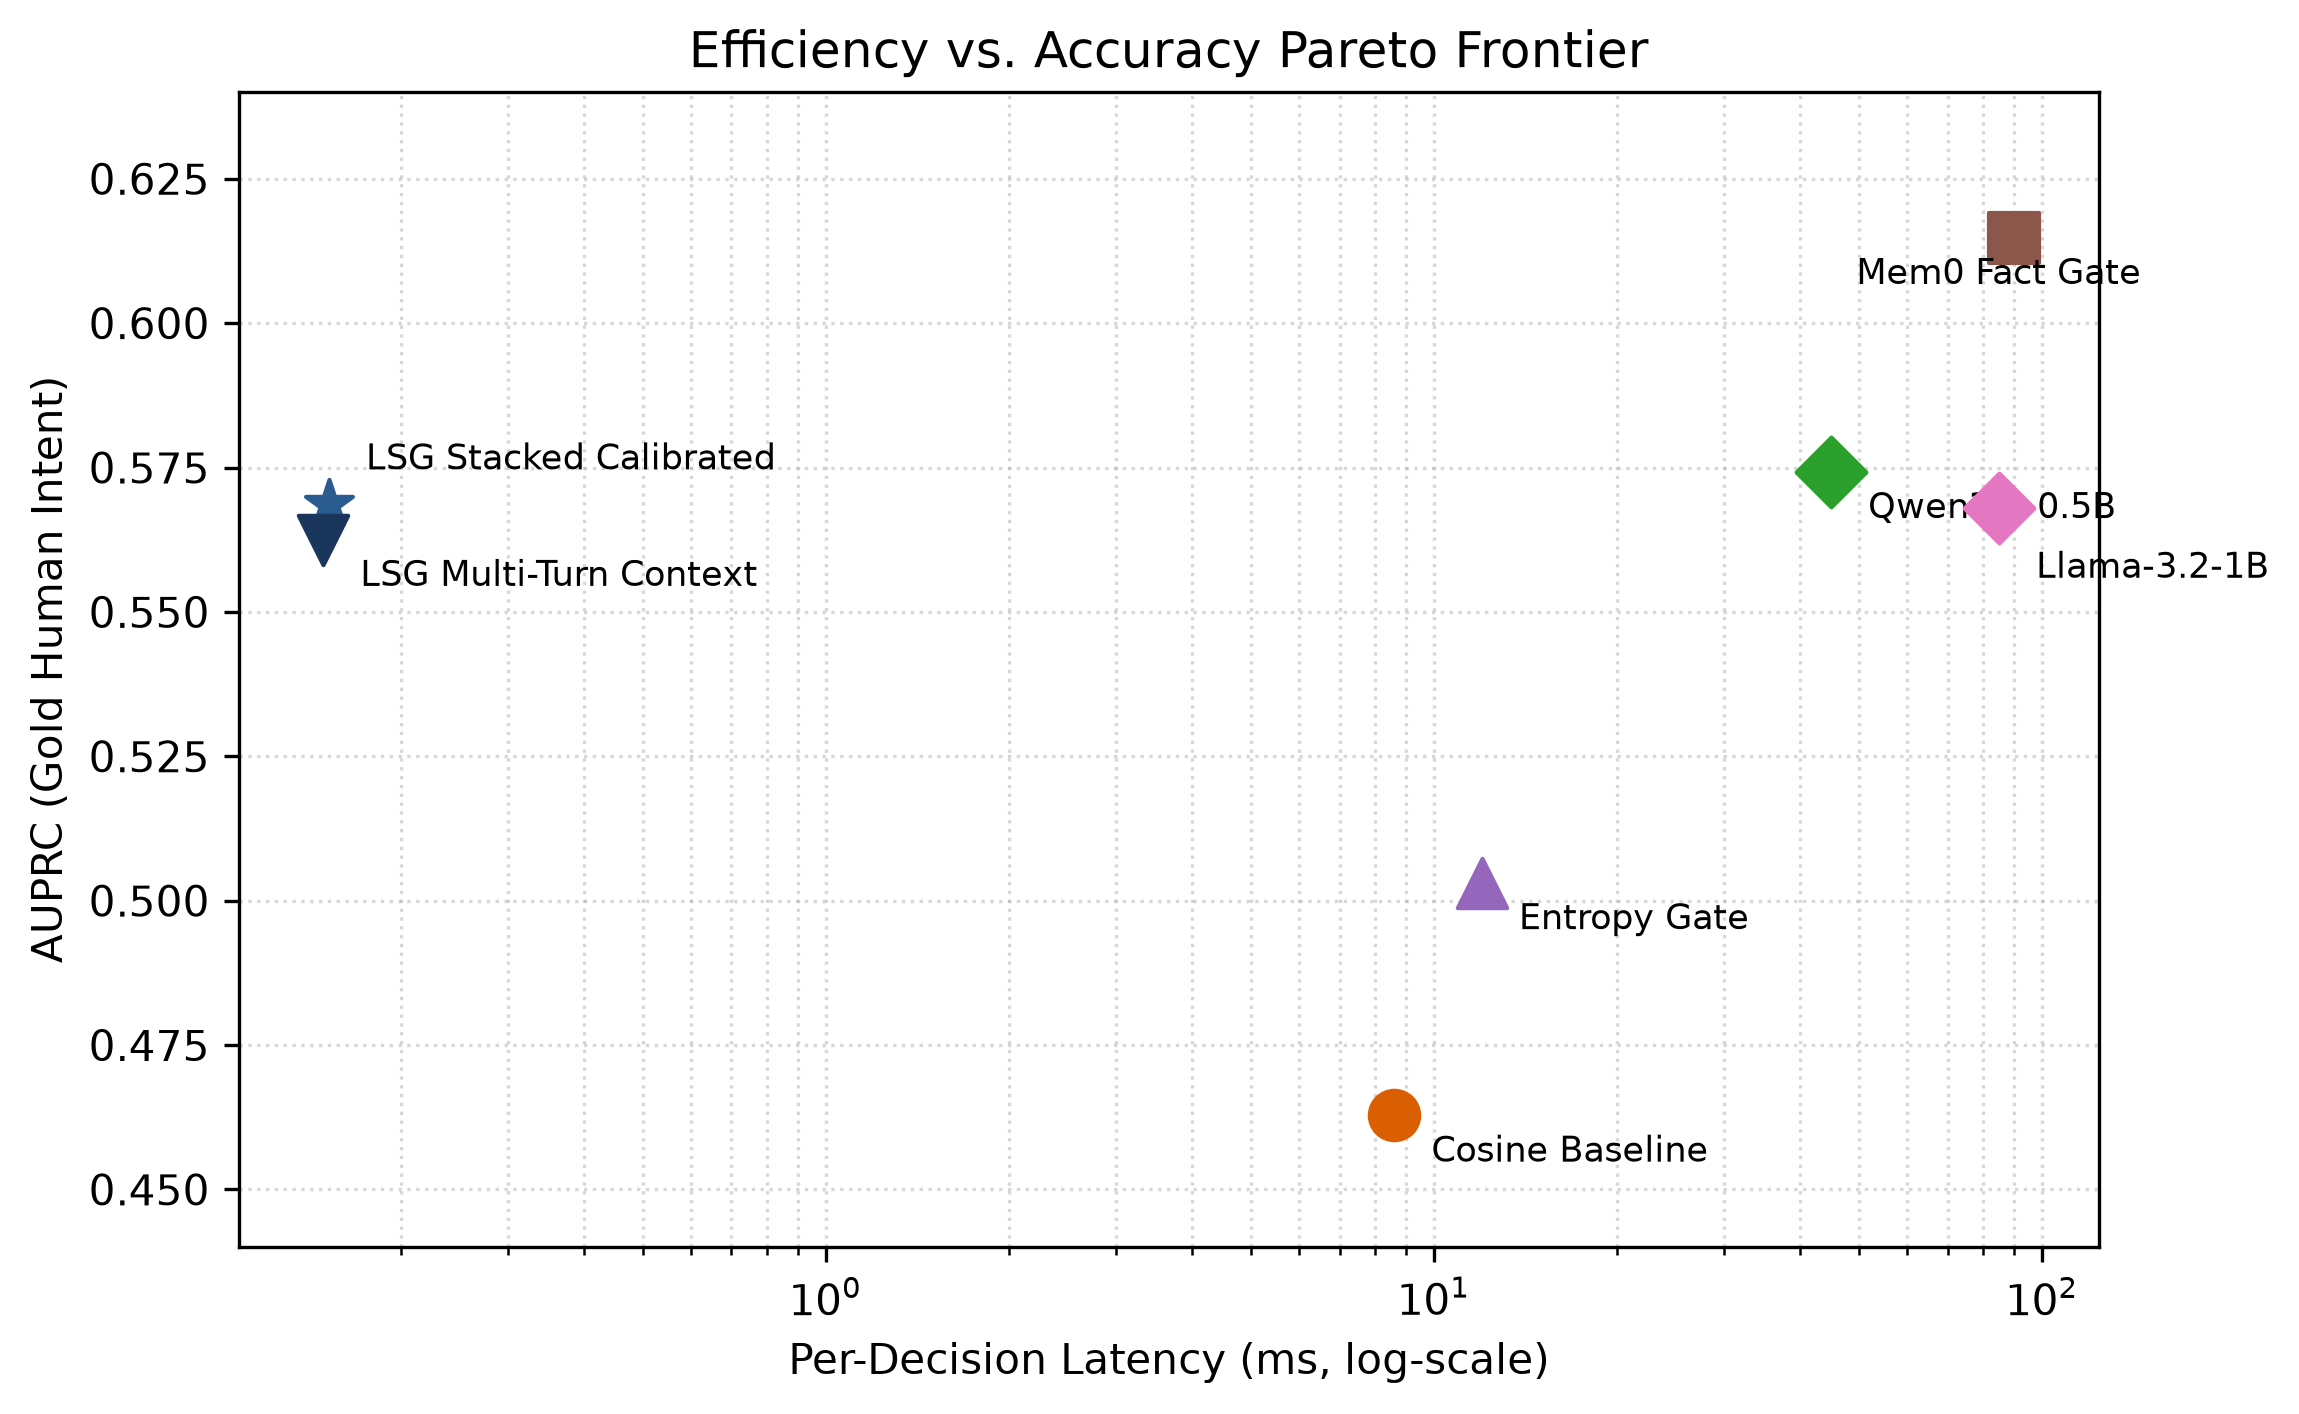
\includegraphics[width=\columnwidth]{figures/pareto_frontier.png}
\caption{Accuracy-Latency Pareto frontier evaluated on the PersonaChat benchmark using gold human intent labels. LSG achieves ranking parity with 0.5B--1B parameter SLMs at sub-millisecond CPU latency.}
\label{fig:pareto}
\end{figure}

\begin{figure}[t]
\centering
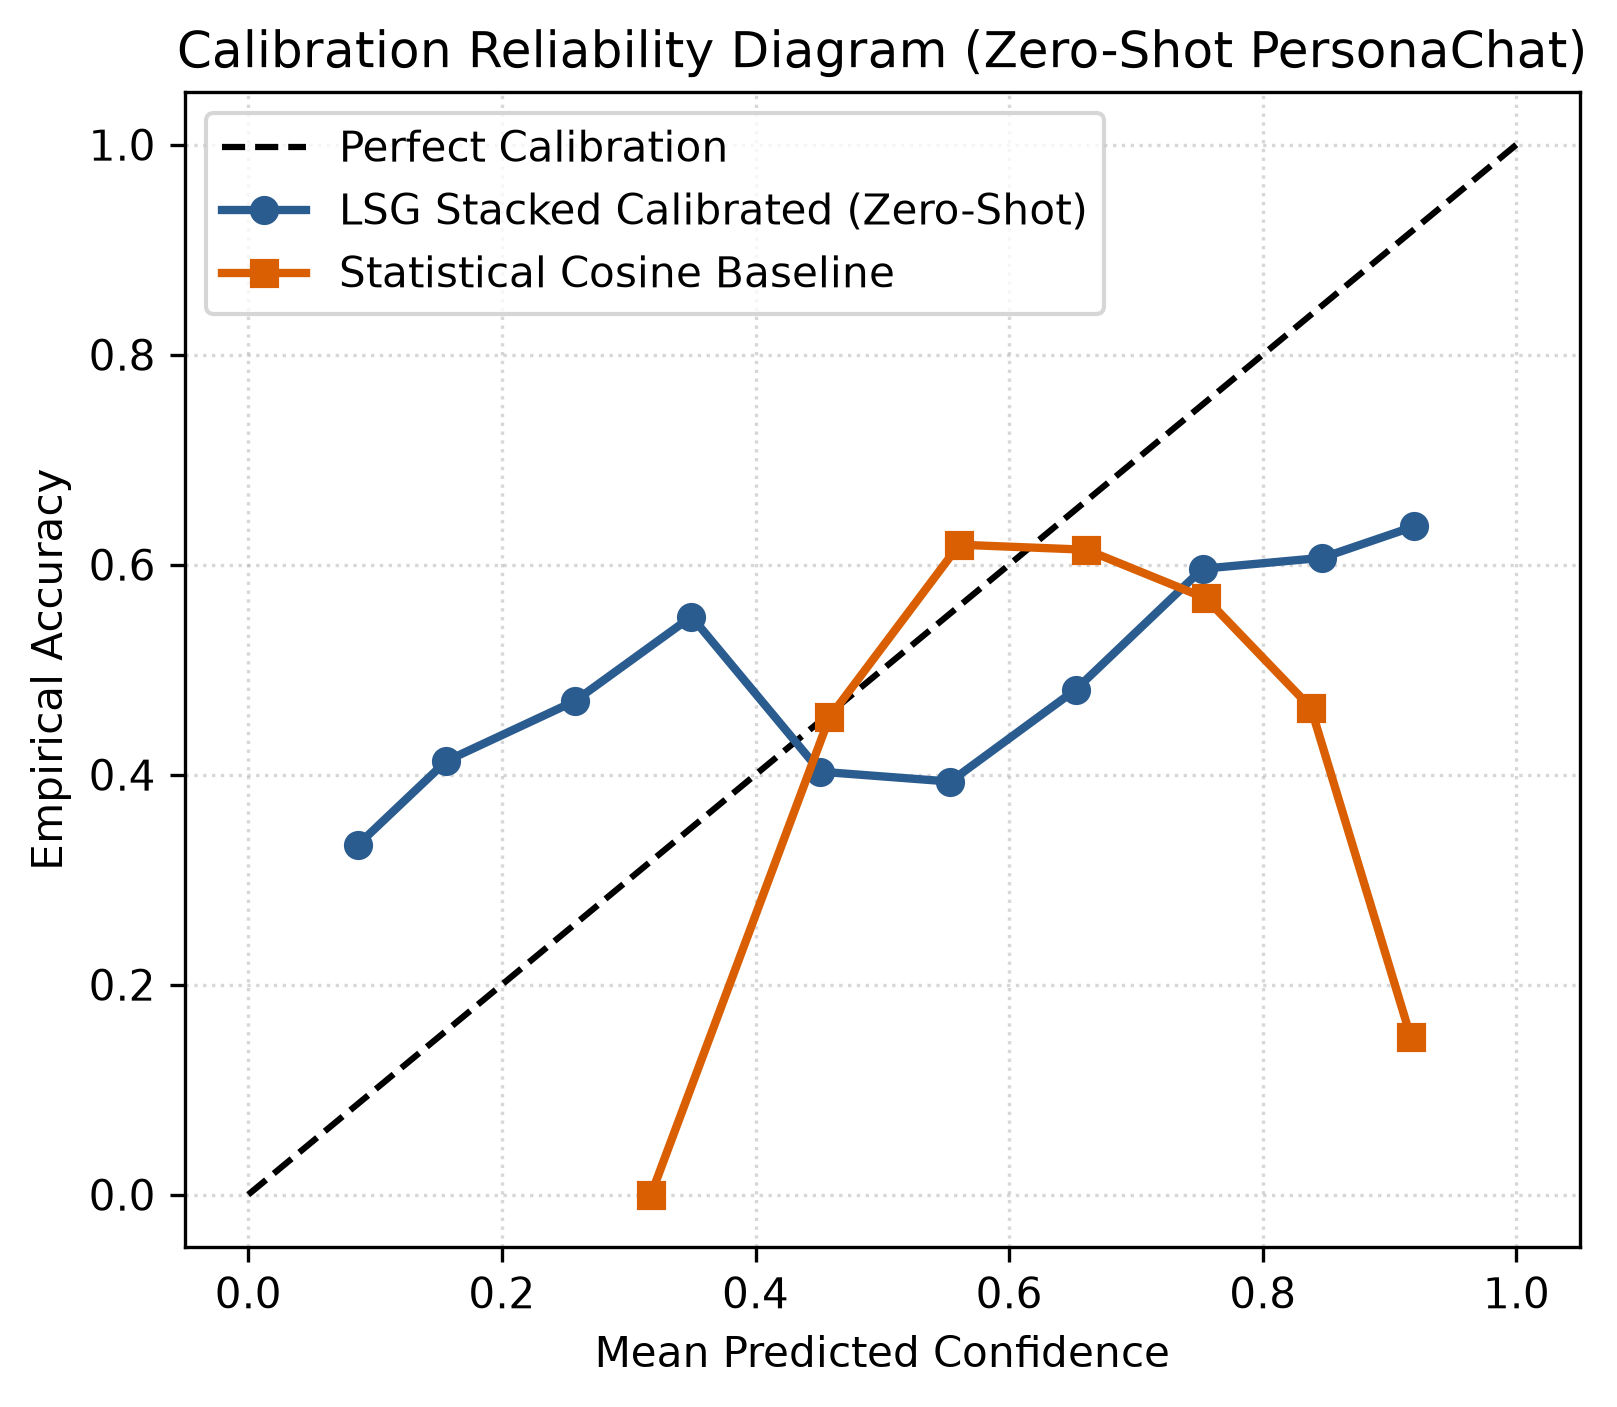
\includegraphics[width=\columnwidth]{figures/calibration_curve.png}
\caption{Empirical calibration reliability diagrams on zero-shot PersonaChat. LSG spans the full probability range $[0.05, 0.96]$, showing monotonic calibration behavior, while the statistical baseline concentrates uncalibrated scores between $0.6$ and $0.9$.}
\label{fig:calibration}
\end{figure}

\subsection{Pareto Frontier and Calibration Reliability}
Fig.~\ref{fig:pareto} plots the empirical Accuracy vs. Latency Pareto frontier using verified benchmark values. The plot demonstrates that LSG establishes a viable operating point on the efficiency frontier: it avoids the $O(N)$ latency and degenerate pass-through failure of cosine thresholds, while bypassing the $45\text{--}90\text{ ms}$ latency penalty of generative SLMs.

Fig.~\ref{fig:calibration} visualizes empirical calibration on the zero-shot PersonaChat test set. The statistical baseline clusters its predictions narrowly within $[0.60, 0.85]$, yielding an apparent $\text{ECE} = 0.238$ simply because its scores fluctuate near the test set prevalence ($52.8\%$). LSG generates calibrated scores spanning the entire interval $[0.05, 0.96]$. However, zero-shot covariate shift causes the ensemble to exhibit overconfidence in high-probability bins, resulting in an empirical $\text{ECE} = 0.401$. While Platt scaling successfully enforces intra-model monotonicity (rectifying non-monotonic probability inversions in the base classifiers), domain shift degrades external probability calibration, demonstrating that target-domain calibration remains essential when moving across dialogue genres.

\section{Limitations and Future Work}
Our findings highlight several clear scope boundaries. First, LSG evaluates write filtering at the turn level. Extending the framework to multi-document agent environments will require evaluating document-level summarization gates. Second, the calibration penalty observed under zero-shot transfer indicates that while shallow ensembles offer fast execution, their probability calibration is sensitive to domain shift, motivating future work on lightweight, unsupervised test-time calibration techniques.

\section{Conclusion}
Write-time memory gating presents a fundamental trade-off in long-horizon LLM agent design. Training-free cosine heuristics exhibit linear $O(N)$ latency scaling and collapse into unselective pass-through filters, while Small Language Models introduce unacceptable per-turn latency. LSG demonstrates that a shallow, Platt-calibrated stacked ensemble can bridge this gap: executing in $0.153\text{ ms}$ on CPU with $O(1)$ complexity, matching the ranking quality of 0.5B--1B parameter SLMs, and eliminating the storage bloat of unselective heuristics. At the same time, our empirical analysis reveals that zero-shot domain transfer incurs a measurable calibration penalty, establishing practical guidelines for deploying lightweight supervised gates in real-time agent architectures.

\bibliographystyle{IEEEtran}
\bibliography{references}

\end{document}
